% cap_fundamentacao.tex
\chapter{Fundamentação Teórica}
\label{chap:fundamentacao_teorica}

Este capítulo apresenta os conceitos necessários para compreender o restante do trabalho. Ele parte da noção de série temporal e explica como uma série é transformada em exemplos de entrada e saída para os modelos. Em seguida, descreve como separar os dados para treinar e avaliar os modelos sem que informação do futuro influencie o resultado, como tratar valores ausentes, como funcionam os modelos utilizados e como medir e comparar a qualidade das previsões.

\section{Séries Temporais}
\label{sec:series_temporais}

Uma série temporal é uma sequência de observações ordenadas no tempo. Neste trabalho, o instante de cada observação é indicado por \(t\), e o valor observado da grandeza de interesse nesse instante é indicado por \(y_t\). Quando a série registra uma única grandeza, ela é chamada de \emph{univariada}: por exemplo, apenas a concentração horária de PM2,5. Quando várias grandezas são registradas nos mesmos instantes, como PM2,5, PM10 e a hora do dia, a série é chamada de \emph{multivariada}. Nesse caso, o conjunto das \(d\) grandezas observadas no instante \(t\) é organizado em um vetor \(\mathbf{x}_t \in \mathbb{R}^{d}\), e o modelo pode usar, além do histórico da grandeza que se deseja prever, o histórico das demais.

Em qualidade do ar, a concentração de um poluente costuma apresentar ciclos diários e semanais, mudanças de comportamento ao longo dos anos, ruído de medição e episódios de concentração elevada. \citeonline{hyndman2021forecasting} descrevem esses padrões como tendência, sazonalidade e variações restantes. Em uma decomposição aditiva simples, o valor observado no instante \(t\) é a soma desses componentes, como mostra a Equação~\ref{eq:decomposicao_aditiva}.

\begin{equation}
    y_t = T_t + S_t + R_t
    \label{eq:decomposicao_aditiva}
\end{equation}

Na Equação~\ref{eq:decomposicao_aditiva}, \(T_t\) é a tendência, isto é, o nível médio da série que varia lentamente; \(S_t\) é a sazonalidade, um padrão que se repete em intervalos fixos, como a cada 24 horas; e \(R_t\) é o restante, que inclui o ruído, as mudanças abruptas e os eventos raros.

Outra medida útil é a autocorrelação, que indica o quanto os valores da série se parecem com os valores anteriores. Para um atraso de \(\ell\) instantes, a autocorrelação amostral de uma série com \(T\) observações é dada pela Equação~\ref{eq:autocorrelacao}.

\begin{equation}
    \rho(\ell)=
    \frac{
        \sum_{t=\ell+1}^{T} (y_t-\bar{y})(y_{t-\ell}-\bar{y})
    }{
        \sum_{t=1}^{T} (y_t-\bar{y})^2
    }
    \label{eq:autocorrelacao}
\end{equation}

Na Equação~\ref{eq:autocorrelacao}, \(y_{t-\ell}\) é o valor observado \(\ell\) instantes antes de \(t\) e \(\bar{y}\) é a média de todos os valores da série. Em uma série horária, \(\rho(1)\) alto indica que o valor de uma hora é parecido com o da hora anterior, \(\rho(24)\) alto indica repetição diária e \(\rho(168)\) alto indica repetição semanal.

\section{Janelas e Variáveis Exógenas}
\label{sec:janelas_variaveis_exogenas}

Os modelos de aprendizado de máquina aprendem a partir de exemplos, cada um formado por uma entrada e pela saída que se espera obter dela. Uma série temporal, porém, é uma única sequência contínua. Para usá-la, ela é dividida em exemplos por meio de uma \emph{janela deslizante} (janelamento): a janela de entrada reúne os \(L\) valores mais recentes até o instante \(t\), e a saída desejada reúne os \(H\) valores seguintes, de \(t+1\) a \(t+H\). O número \(L\) é o comprimento da janela de entrada, e \(H\) é o horizonte de previsão, isto é, quantos instantes à frente se deseja prever. Ao avançar a janela um instante de cada vez, obtém-se um novo exemplo a cada passo.

A Figura~\ref{fig:janelamento} ilustra o procedimento com \(L=3\) e \(H=2\). Observe que cada linha é a mesma série, e que as caixas azuis mostram a entrada e as caixas laranja mostram a saída desejada. Na amostra 1, a entrada é formada por \(y_1\), \(y_2\) e \(y_3\), e a saída desejada por \(y_4\) e \(y_5\). Na amostra 2, a janela avança uma posição: a entrada passa a ser \(y_2\), \(y_3\) e \(y_4\), e a saída desejada, \(y_5\) e \(y_6\). Como as janelas se sobrepõem, o mesmo valor aparece em vários exemplos, ora como entrada, ora como saída.

\begin{figure}[htbp]
    \centering
    \begin{tikzpicture}[x=0.95cm,y=0.95cm,box/.style={draw,minimum size=0.8cm,inner sep=0,font=\small}]
        \foreach \s in {1,2,3}{
            \node[anchor=east,font=\small] at (0.4,{3.4-\s}) {Amostra \s};
            \foreach \i in {1,...,9}{
                \pgfmathtruncatemacro{\a}{\i-\s}
                \ifnum\a<0 \def\cor{white}\else\ifnum\a<3 \def\cor{blue!30}\else\ifnum\a<5 \def\cor{orange!45}\else\def\cor{white}\fi\fi\fi
                \node[box,fill=\cor] at (\i,{3.4-\s}) {$y_{\i}$};
            }
        }
        \draw[-{Latex[length=2.5mm]}] (0.6,0) -- (9.8,0) node[right,font=\small] {tempo};
        \node[box,fill=blue!30] at (2.2,-0.9) {};
        \node[anchor=west,font=\small] at (2.7,-0.9) {entrada (\(L=3\) valores)};
        \node[box,fill=orange!45] at (6.2,-0.9) {};
        \node[anchor=west,font=\small] at (6.7,-0.9) {saída desejada (\(H=2\) valores)};
    \end{tikzpicture}
    \caption{Janela deslizante sobre uma série, com \(L=3\) valores de entrada e \(H=2\) valores de saída. A cada amostra a janela avança um instante. Elaboração própria.}
    \label{fig:janelamento}
\end{figure}

Formalmente, seja \(\mathbf{x}_t \in \mathbb{R}^{d}\) o vetor das variáveis observadas no instante \(t\) e \(y_t\) o valor de interesse nesse mesmo instante. Alguns atributos, além disso, são conhecidos de antemão para os instantes futuros, como a hora do dia; eles formam o vetor \(\mathbf{z}_{t+k}\), com \(k=1,\ldots,H\). Um modelo \(f_{\theta}\), cujos parâmetros são reunidos em \(\theta\), transforma uma janela de entrada em uma previsão, conforme a Equação~\ref{eq:janela_supervisionada}.

\begin{equation}
    \hat{\mathbf{y}}_{t+1:t+H}
    =
    f_{\theta}\left(
        \mathbf{x}_{t-L+1:t},
        \mathbf{z}_{t+1:t+H}
    \right)
    \label{eq:janela_supervisionada}
\end{equation}

Na Equação~\ref{eq:janela_supervisionada}, \(\mathbf{x}_{t-L+1:t}\) é a janela de entrada, formada pelos vetores dos instantes \(t-L+1\) até \(t\); \(\mathbf{z}_{t+1:t+H}\) reúne os atributos conhecidos de antemão para o horizonte; e \(\hat{\mathbf{y}}_{t+1:t+H}=(\hat{y}_{t+1},\ldots,\hat{y}_{t+H})\) é a sequência prevista. O acento circunflexo indica que o valor é uma previsão, e não uma observação. O treinamento consiste em ajustar \(\theta\) para que \(\hat{\mathbf{y}}\) se aproxime dos valores observados.

Algumas definições completam essa formulação. \emph{Defasagem} é o uso de um valor passado de uma variável como atributo, como a concentração observada 24 horas antes. \emph{Variável exógena} é uma variável externa ao valor que se quer prever, como o PM10 ou a temperatura, quando usadas para prever o PM2,5. \emph{Atributos de calendário} descrevem o instante de forma conhecida com antecedência, como a hora do dia, o dia da semana e o mês. \emph{Termos periódicos} representam um ciclo por meio de funções seno e cosseno, como mostra a Equação~\ref{eq:termos_periodicos}, para um período \(P\) (por exemplo, \(P=24\) horas).

\begin{equation}
    s(t)=\sin\left(\frac{2\pi t}{P}\right),
    \qquad
    c(t)=\cos\left(\frac{2\pi t}{P}\right)
    \label{eq:termos_periodicos}
\end{equation}

Na Equação~\ref{eq:termos_periodicos}, \(s(t)\) e \(c(t)\) variam continuamente ao longo do ciclo e voltam ao mesmo valor a cada \(P\) instantes. Com isso, as 23 horas e a 0 hora, que são vizinhas no relógio, também ficam próximas na representação numérica, o que não ocorreria se a hora fosse usada como número de 0 a 23.

Uma variável só pode servir de atributo para um instante futuro se seu valor já for conhecido no momento em que a previsão é emitida. Calendário e termos periódicos satisfazem essa condição. O PM10 medido em \(t+5\), por exemplo, não a satisfaz: usá-lo daria ao modelo uma informação que não existiria na prática. Esse problema é discutido na Seção~\ref{sec:dados_faltantes_imputacao}.

\section{Previsão Multi-Horizonte}
\label{sec:previsao_multi_horizonte}

Na previsão multi-horizonte, o modelo estima vários instantes futuros a partir do mesmo instante de emissão \(t\), e não apenas o próximo \cite{lim2021survey,benidis2022deep}. Três estratégias são usadas para isso.

\begin{itemize}
    \item \textbf{Recursiva:} o modelo aprende a prever apenas um instante à frente, \(\hat{y}_{t+1}=g_{\theta}(\mathbf{x}_{t-L+1:t})\), e a previsão obtida é reinserida na entrada para se obter \(\hat{y}_{t+2}\), e assim por diante até \(\hat{y}_{t+H}\). Essa estratégia é usada, por exemplo, pelo DeepAR \cite{salinas2020deepar}. Sua desvantagem é que o erro de uma previsão se propaga para as seguintes.
    \item \textbf{Direta:} o modelo produz cada horizonte sem depender das previsões anteriores. Isso pode ser feito com um modelo independente para cada horizonte, \(\hat{y}_{t+h}=g_{\theta}^{(h)}(\mathbf{x}_{t-L+1:t})\), ou com um único modelo de \(H\) saídas \cite{taieb2012review}. Um exemplo é o MQ-RNN (\textit{Multi-horizon Quantile Recurrent Neural Network}) \cite{wen2017mqrnn}, que produz os vários horizontes de uma só vez.
    \item \textbf{Codificador-decodificador:} uma parte do modelo, o codificador, resume a janela de entrada; outra parte, o decodificador, gera a sequência prevista a partir desse resumo. O \textit{Temporal Fusion Transformer} \cite{lim2021tft}, por exemplo, contém uma camada desse tipo. Esta arquitetura é detalhada na Seção~\ref{sec:encoder_decoder_attention}.
\end{itemize}

Nenhuma estratégia é superior em todos os casos: a literatura de previsão não indica uma arquitetura dominante, e revisões de redes recorrentes para séries temporais afirmam que não há solução universal \cite{hewamalage2021rnn}. Por isso, a escolha precisa ser verificada em cada problema.

\section{Validação Temporal}
\label{sec:validacao_temporal}

Para saber se um modelo prevê bem, é preciso avaliá-lo em dados que ele não viu durante o treinamento. Por isso, os dados são divididos em três conjuntos. O conjunto de \emph{treino} é usado para ajustar os parâmetros do modelo. O conjunto de \emph{validação} é usado para comparar configurações do modelo e escolher a melhor, sem alterar os parâmetros. O conjunto de \emph{teste} é reservado desde o início e usado apenas no final, para estimar a qualidade da previsão em dados novos.

Em séries temporais, essa divisão deve respeitar a ordem cronológica: o treino vem antes da validação, e esta, antes do teste. Uma divisão aleatória misturaria instantes de períodos diferentes, e o modelo poderia aprender com valores posteriores aos que precisa prever, o que dá uma estimativa otimista demais da qualidade \cite{hyndman2021forecasting,tashman2000out,bergmeir2012crossvalidation}.

A validação cruzada tradicional repete a avaliação em várias divisões dos dados e faz a média dos resultados, mas supõe exemplos independentes entre si, o que não vale para observações vizinhas de uma série. Uma adaptação usual é a validação por janela expansiva (\textit{walk-forward}). A Figura~\ref{fig:validacao_walk_forward} ilustra o procedimento com três partições. Observe que, na partição 1, o treino ocupa o bloco 1 e a validação ocupa o bloco 2. Na partição 2, o treino passa a ocupar os blocos 1 e 2, e a validação, o bloco 3. Na partição 3, o treino ocupa os blocos 1 a 3, e a validação, o bloco 4. Em todas as partições, a validação vem depois do treino, e o bloco final, em verde, permanece separado como conjunto de teste, sem participar de nenhuma escolha.

\begin{figure}[htbp]
    \centering
    \begin{tikzpicture}[x=1.9cm,y=1cm,every node/.style={font=\small}]
        \foreach \b/\t in {0/Bloco 1,1/Bloco 2,2/Bloco 3,3/Bloco 4,4/Bloco final}{
            \node at ({\b+0.5},0.8) {\t};
        }
        \draw[-{Latex[length=2.5mm]}] (0,0.35) -- (5.15,0.35) node[right] {tempo};
        \foreach \p/\n in {1/2,2/3,3/4}{
            \pgfmathtruncatemacro{\q}{\p+1}
            \node[anchor=east] at (-0.1,{-0.6*\p}) {Partição \p};
            \fill[blue!30,draw=blue!60!black] (0.03,{-0.6*\p-0.22}) rectangle ({\p-0.03},{-0.6*\p+0.22});
            \node at ({\p/2},{-0.6*\p}) {treino};
            \fill[orange!45,draw=orange!70!black] ({\p+0.03},{-0.6*\p-0.22}) rectangle ({\q-0.03},{-0.6*\p+0.22});
            \node at ({\p+0.5},{-0.6*\p}) {validação};
            \fill[green!35,draw=green!50!black] (4.03,{-0.6*\p-0.22}) rectangle (4.97,{-0.6*\p+0.22});
            \node at (4.5,{-0.6*\p}) {teste};
        }
    \end{tikzpicture}
    \caption{Validação por janela expansiva com três partições. Em cada partição, o treino usa apenas dados anteriores à validação, e o bloco final fica reservado para o teste. Elaboração própria, com base em \citeonline{tashman2000out}, \citeonline{bergmeir2012crossvalidation} e \citeonline{hyndman2021forecasting}.}
    \label{fig:validacao_walk_forward}
\end{figure}

Para \(K\) partições, o resultado usado para comparar configurações é a média das medidas de erro obtidas na validação de cada partição, como mostra a Equação~\ref{eq:cv_temporal}.

\begin{equation}
    \mathcal{L}_{CV}
    =
    \frac{1}{K}\sum_{k=1}^{K}
    \mathcal{L}_{val}^{(k)}
    \label{eq:cv_temporal}
\end{equation}

Na Equação~\ref{eq:cv_temporal}, \(\mathcal{L}_{val}^{(k)}\) é a medida de erro obtida na validação da partição \(k\), e \(\mathcal{L}_{CV}\) é a média entre as \(K\) partições (o índice \(CV\) vem de \textit{cross-validation}, validação cruzada).

\section{Dados Faltantes, Imputação e Vazamento Temporal}
\label{sec:dados_faltantes_imputacao}

\subsection{Dados faltantes}

Dados ambientais reais frequentemente apresentam lacunas, isto é, instantes em que a medição esperada não foi registrada. As causas incluem falhas do sensor, manutenção, problemas de comunicação e descarte de leituras inconsistentes. \citeonline{littlerubin2019statistical} distinguem os casos conforme o motivo da ausência: ela pode ser independente dos valores (por exemplo, uma queda de energia), depender de outras variáveis observadas, ou depender do próprio valor que deixou de ser medido (por exemplo, um sensor que falha justamente quando a concentração é alta). No último caso, a ausência carrega informação sobre o valor perdido e é mais difícil de tratar.

\subsection{Imputação}

Imputação é o preenchimento das lacunas com valores estimados, o que permite formar janelas completas para o modelo. Os métodos mais simples repetem o último valor observado ou fazem uma interpolação linear entre o valor anterior e o posterior à lacuna. Métodos multivariados, como a imputação multivariada por equações encadeadas (\textit{Multivariate Imputation by Chained Equations}, MICE) e o MissForest, estimam o valor faltante a partir das demais variáveis \cite{vanbuuren2011mice,stekhoven2012missforest}. Um valor imputado é uma estimativa e não uma medição. Uma forma de manter essa distinção é acrescentar ao modelo um indicador de ausência, uma variável que vale 1 quando o valor original estava faltando e 0 quando foi medido \cite{che2018recurrent}.

\subsection{Vazamento temporal}

Vazamento temporal ocorre quando uma etapa de preparação dos dados usa informação que não estaria disponível no instante real da previsão. Três exemplos ilustram o problema. No primeiro, a média e o desvio-padrão usados para normalizar a série (colocar as variáveis em escala comparável) são calculados com todos os dados, inclusive os de validação e de teste, de modo que estatísticas do futuro influenciam o treinamento. No segundo, uma lacuna na validação é preenchida por interpolação linear usando uma medição posterior à origem da previsão. No terceiro, um atributo como a média das últimas 24 horas é calculado incluindo horas posteriores ao instante de emissão.

Para evitar o vazamento, a normalização, a imputação e a criação de atributos devem ser ajustadas apenas com dados anteriores ao período que será avaliado. Em uma validação por janela expansiva, por exemplo, a média e o desvio-padrão são calculados no bloco de treino de cada partição e depois aplicados ao bloco de validação; e as lacunas da validação não podem ser preenchidas com medições posteriores ao instante em que a previsão seria feita. Variáveis futuras só podem ser usadas quando forem conhecidas antes da previsão, como o calendário.

\section{Redes Neurais e Aprendizado Profundo}
\label{sec:redes_neurais_deep_learning}

Redes neurais artificiais são modelos formados por unidades simples, chamadas neurônios, conectadas por pesos. A inspiração histórica vem de modelos matemáticos do neurônio biológico, como o de \citeonline{mcculloch1943logical} e o perceptron de \citeonline{rosenblatt1958perceptron}. Trata-se de uma analogia: as redes usadas em aprendizado de máquina não reproduzem a fisiologia dos neurônios reais, apenas a ideia de combinar entradas, ponderá-las e produzir uma saída. Em um neurônio biológico, os dendritos recebem sinais, o corpo celular integra parte deles e o axônio transmite o resultado a outras células; o neurônio artificial mantém a ideia de entradas ponderadas, soma e resposta (Figura~\ref{fig:neuronio_biologico_artificial}).

\begin{figure}[htbp]
    \centering
    \begin{subfigure}[t]{0.42\linewidth}
        \centering
        \includegraphics[width=\linewidth,trim=100 500 320 520,clip]{neuronio-biologico-wikimedia-ptbr.png}
        \caption{Neurônio biológico.}
        \label{fig:neuronio_biologico}
    \end{subfigure}
    \hfill
    \begin{subfigure}[t]{0.54\linewidth}
        \centering
        \includegraphics[width=\linewidth]{diagrama_neuronio_artificial_proprio.pdf}
        \caption{Neurônio artificial.}
        \label{fig:neuronio_artificial_perceptron}
    \end{subfigure}
    \caption[Neurônio biológico e neurônio artificial]{Comparação entre o neurônio biológico e o neurônio artificial. A imagem do neurônio biológico, com rótulos em português, foi obtida de \citeonline{vasconcelos2008neuronPt}; a representação do neurônio artificial é elaboração própria, adaptada de \citeonline{tzanis2021representativePM}.}
    \label{fig:neuronio_biologico_artificial}
\end{figure}

Na Figura~\ref{fig:neuronio_artificial_perceptron}, observe que cada entrada \(x_j\) é multiplicada por um peso \(w_j\), que os produtos são somados junto com o viés \(b\) (um valor constante que desloca o resultado) e que a soma passa por uma função de ativação \(\phi\), que produz a saída \(\hat{y}\). A Equação~\ref{eq:neuronio_artificial} expressa exatamente essas operações.

\begin{equation}
    a = \sum_{j=1}^{d} w_jx_j + b,
    \qquad
    \hat{y} = \phi(a)
    \label{eq:neuronio_artificial}
\end{equation}

Na Equação~\ref{eq:neuronio_artificial}, \(d\) é o número de entradas, \(a\) é a soma ponderada e \(\phi\) é a função de ativação, que introduz não linearidade e permite à rede representar relações que não são retas. Exemplos de função de ativação são a sigmoide, \(\sigma(a)=1/(1+e^{-a})\), que devolve valores entre 0 e 1, e a tangente hiperbólica, \(\tanh(a)\), que devolve valores entre \(-1\) e 1. Neste texto, \(\hat{y}\) é sempre a previsão produzida pela camada final da rede, e \(\mathbf{h}\) é o vetor de saídas de uma camada intermediária.

Uma rede neural organiza vários neurônios em camadas: as saídas de uma camada são as entradas da camada seguinte. A camada de índice \(\ell\) é descrita pela Equação~\ref{eq:camada_neural}.

\begin{equation}
    \mathbf{h}^{(\ell)}
    =
    \phi\left(
        W^{(\ell)}\mathbf{h}^{(\ell-1)}
        +
        \mathbf{b}^{(\ell)}
    \right)
    \label{eq:camada_neural}
\end{equation}

Na Equação~\ref{eq:camada_neural}, \(\mathbf{h}^{(\ell-1)}\) é o vetor de saídas da camada anterior (na primeira camada, é a própria entrada), \(W^{(\ell)}\) é a matriz cujos elementos são os pesos da camada \(\ell\), \(\mathbf{b}^{(\ell)}\) é o vetor de vieses e \(\mathbf{h}^{(\ell)}\) é a saída da camada. O treinamento ajusta pesos e vieses para reduzir a \emph{perda}, um número que mede a distância entre as previsões e os valores observados. Para isso, calcula-se o gradiente da perda, isto é, a derivada da perda em relação a cada parâmetro, que indica em que direção e com que intensidade alterá-lo para reduzir a perda; a retropropagação é o procedimento que calcula esses gradientes camada por camada, da saída para a entrada \cite{goodfellow2016deep}.

Aprendizado profundo (\textit{deep learning}) é o treinamento de redes neurais com várias camadas, em que cada camada produz uma representação mais elaborada dos dados \cite{goodfellow2016deep,lecun2015deep}. Ele é um caso particular do aprendizado de máquina.

\section{Redes Neurais Recorrentes e \textit{Long Short-Term Memory}}
\label{sec:rnn_lstm}

Redes neurais recorrentes (\textit{Recurrent Neural Networks}, RNNs) são projetadas para sequências. Elas leem a sequência um instante de cada vez e mantêm um \emph{estado interno}, um vetor \(\mathbf{h}_t\) que resume o que foi lido até o instante \(t\) e é repassado ao passo seguinte. Esse estado também é chamado de estado oculto. Em uma RNN simples, ele é calculado pela Equação~\ref{eq:rnn}.

\begin{equation}
    \mathbf{h}_t = \tanh\left(W\mathbf{x}_t + U\mathbf{h}_{t-1} + \mathbf{b}\right)
    \label{eq:rnn}
\end{equation}

Na Equação~\ref{eq:rnn}, \(\mathbf{x}_t\) é a entrada no instante \(t\), \(\mathbf{h}_{t-1}\) é o estado do passo anterior, \(W\) e \(U\) são matrizes de pesos e \(\mathbf{b}\) é o vetor de vieses. A Figura~\ref{fig:rnn_desdobrada} mostra a mesma rede repetida em três instantes: observe que o estado \(\mathbf{h}_t\) depende da entrada \(\mathbf{x}_t\) e do estado anterior, de modo que a informação dos primeiros instantes chega aos últimos por uma cadeia de cálculos.

\begin{figure}[htbp]
    \centering
    \begin{tikzpicture}[x=2.6cm,y=1.2cm,cell/.style={draw,rounded corners,minimum width=1.5cm,minimum height=0.8cm,fill=blue!10},every node/.style={font=\small}]
        \foreach \i/\lab in {0/{t-1},1/{t},2/{t+1}}{
            \node[cell] (c\i) at (\i,0) {RNN};
            \node (x\i) at (\i,-1.3) {\(\mathbf{x}_{\lab}\)};
            \node (h\i) at (\i,1.3) {\(\mathbf{h}_{\lab}\)};
            \draw[-{Latex[length=2mm]}] (x\i) -- (c\i);
            \draw[-{Latex[length=2mm]}] (c\i) -- (h\i);
        }
        \draw[-{Latex[length=2mm]}] (c0) -- (c1);
        \draw[-{Latex[length=2mm]}] (c1) -- (c2);
        \draw[-{Latex[length=2mm]}] (-0.75,0) -- (c0);
        \draw[-{Latex[length=2mm]}] (c2) -- (2.75,0);
    \end{tikzpicture}
    \caption{Rede recorrente desdobrada em três instantes. A seta horizontal transporta o estado interno de um passo para o seguinte. Elaboração própria.}
    \label{fig:rnn_desdobrada}
\end{figure}

Em RNNs simples, o treinamento sofre com o desaparecimento ou a explosão de gradientes. Como o gradiente em um instante inicial é obtido multiplicando muitos fatores, um por passo de tempo, ele tende a ficar muito pequeno quando esses fatores são menores que 1 (desaparecimento) ou muito grande quando são maiores que 1 (explosão). No primeiro caso, o modelo praticamente deixa de aprender com o início da sequência, o que dificulta capturar dependências longas.

A rede de memória de curto e longo prazo (\textit{Long Short-Term Memory}, LSTM) foi proposta para reduzir esse problema \cite{hochreiter1997long}. Ela acrescenta uma célula de memória, um vetor \(\mathbf{c}_t\) que atravessa a sequência com poucas alterações, e três \emph{portões} (\textit{gates}). Cada portão é um vetor de valores entre 0 e 1, obtido com a função sigmoide, que multiplica outro vetor elemento a elemento e funciona como uma válvula: valores próximos de 0 bloqueiam a informação, e valores próximos de 1 a deixam passar. O portão de esquecimento decide quanto da memória anterior é mantido; o portão de entrada decide quanto do novo conteúdo é gravado; e o portão de saída decide quanto da memória é exposto como estado oculto.

A Figura~\ref{fig:lstm_cell} mostra a estrutura de uma célula no instante \(t\). Observe a linha superior, que carrega a memória de \(\mathbf{c}_{t-1}\) para \(\mathbf{c}_t\), e a linha inferior, que recebe a entrada atual \(\mathbf{x}_t\) e o estado oculto anterior \(\mathbf{h}_{t-1}\). O primeiro bloco sigmoide é o portão de esquecimento (\(F_t\) na figura, \(\mathbf{f}_t\) na Equação~\ref{eq:lstm}). O segundo bloco sigmoide é o portão de entrada (\(I_t\) na figura, \(\mathbf{i}_t\) na equação), e o bloco \(\tanh\) ao lado produz o conteúdo candidato \(\tilde{\mathbf{c}}_t\). O bloco sigmoide à direita é o portão de saída (\(O_t\) na figura, \(\mathbf{o}_t\) na equação). Os círculos rosa da figura, \(o_{t-1}\), \(o_t\) e \(o_{t+1}\), são as saídas da rede em cada instante e, nesta equação, correspondem ao estado oculto \(\mathbf{h}_t\); eles não são o portão de saída.

\begin{figure}[htbp]
    \centering
    \includegraphics[width=0.78\textwidth]{lstm_fdeloche_wikimedia.png}
    \caption[Estrutura interna de uma célula LSTM]{Estrutura interna de uma célula LSTM, com memória, estado oculto, portões e operações elemento a elemento. Fonte: \citeonline{fdeloche2017lstmCell}.}
    \label{fig:lstm_cell}
\end{figure}

A célula LSTM é descrita pela Equação~\ref{eq:lstm}.

\begin{equation}
\begin{aligned}
    \mathbf{f}_t &= \sigma(W_f\mathbf{x}_t + U_f\mathbf{h}_{t-1} + \mathbf{b}_f),\\
    \mathbf{i}_t &= \sigma(W_i\mathbf{x}_t + U_i\mathbf{h}_{t-1} + \mathbf{b}_i),\\
    \tilde{\mathbf{c}}_t &= \tanh(W_c\mathbf{x}_t + U_c\mathbf{h}_{t-1} + \mathbf{b}_c),\\
    \mathbf{o}_t &= \sigma(W_o\mathbf{x}_t + U_o\mathbf{h}_{t-1} + \mathbf{b}_o),\\
    \mathbf{c}_t &= \mathbf{f}_t \odot \mathbf{c}_{t-1} + \mathbf{i}_t \odot \tilde{\mathbf{c}}_t,\\
    \mathbf{h}_t &= \mathbf{o}_t \odot \tanh(\mathbf{c}_t).
\end{aligned}
\label{eq:lstm}
\end{equation}

Na Equação~\ref{eq:lstm}, \(\sigma\) é a função sigmoide, \(\tanh\) é a tangente hiperbólica e \(\odot\) indica multiplicação elemento a elemento. As matrizes \(W\) e \(U\) e os vetores \(\mathbf{b}\) são parâmetros aprendidos no treinamento. As quatro primeiras linhas calculam os três portões e o conteúdo candidato. A quinta linha atualiza a memória: o portão de esquecimento \(\mathbf{f}_t\) mantém parte da memória anterior e o portão de entrada \(\mathbf{i}_t\) grava parte do conteúdo candidato. A última linha produz o estado oculto \(\mathbf{h}_t\), com a parcela da memória que o portão de saída \(\mathbf{o}_t\) deixa passar.

\section{\textit{Sequence-to-Sequence} e Atenção}
\label{sec:encoder_decoder_attention}

Os modelos sequência-para-sequência (\textit{Sequence-to-Sequence}, Seq2Seq) foram propostos para transformar uma sequência de entrada em uma sequência de saída de outro comprimento \cite{sutskever2014sequence}. Eles têm duas partes. O codificador é uma rede recorrente que lê a entrada e produz uma sequência de estados \(\mathbf{h}_1,\ldots,\mathbf{h}_L\), como mostra a Equação~\ref{eq:seq2seq_encoder}. O decodificador é outra rede recorrente que gera a saída um elemento por vez. Na previsão, a janela de entrada é a sequência de entrada, e o horizonte previsto é a sequência de saída.

\begin{equation}
    \mathbf{h}_j = \mathrm{Enc}_{\theta}(\mathbf{x}_{t-L+j}, \mathbf{h}_{j-1}),
    \qquad
    j=1,\ldots,L
    \label{eq:seq2seq_encoder}
\end{equation}

Na Equação~\ref{eq:seq2seq_encoder}, \(\mathrm{Enc}_{\theta}\) é a rede recorrente do codificador (por exemplo, uma LSTM), \(\mathbf{x}_{t-L+j}\) é a entrada do passo \(j\) da janela e \(\mathbf{h}_{j-1}\) é o estado do passo anterior. Na versão original, o decodificador recebe apenas o último estado do codificador, que precisa resumir toda a janela em um único vetor. Esse vetor único é um gargalo, e \citeonline{bahdanau2014neural} propuseram a atenção para reduzi-lo: a cada passo de saída \(k\), o decodificador calcula uma média ponderada de todos os estados do codificador, em que os pesos indicam quais instantes da entrada são mais importantes para aquele passo.

A Figura~\ref{fig:seq2seq_atencao} apresenta esse esquema, adaptado da figura original de \citeonline{bahdanau2014neural}. Observe que, na parte inferior, o codificador produz um estado \(\mathbf{h}_j\) para cada entrada \(\mathbf{x}_j\). Cada estado é multiplicado por um peso de atenção \(\alpha_{k,j}\), e a soma ponderada forma o contexto \(\mathbf{c}_k\), que entra no decodificador junto com seu estado anterior \(\mathbf{s}_{k-1}\) para produzir o novo estado \(\mathbf{s}_k\) e a previsão \(\hat{y}_{t+k}\).

\begin{figure}[htbp]
    \centering
    \resizebox{0.98\linewidth}{!}{%
    \begin{tikzpicture}[every node/.style={font=\small},
        enc/.style={draw,rounded corners,minimum width=1.2cm,minimum height=0.8cm,fill=blue!12},
        dec/.style={draw,rounded corners,minimum width=1.4cm,minimum height=0.8cm,fill=orange!25}]
        \node[enc] (e1) at (0,0) {\(\mathbf{h}_{1}\)};
        \node[enc] (e2) at (2,0) {\(\mathbf{h}_{2}\)};
        \node (ed) at (4,0) {\(\cdots\)};
        \node[enc] (eL) at (6,0) {\(\mathbf{h}_{L}\)};
        \node (x1) at (0,-1.5) {\(\mathbf{x}_{1}\)};
        \node (x2) at (2,-1.5) {\(\mathbf{x}_{2}\)};
        \node (xd) at (4,-1.5) {\(\cdots\)};
        \node (xL) at (6,-1.5) {\(\mathbf{x}_{L}\)};
        \draw[-{Latex[length=2.5mm]}] (x1) -- (e1);
        \draw[-{Latex[length=2.5mm]}] (x2) -- (e2);
        \draw[-{Latex[length=2.5mm]}] (xL) -- (eL);
        \draw[-{Latex[length=2.5mm]}] (e1) -- (e2);
        \draw[-{Latex[length=2.5mm]}] (e2) -- (3.5,0);
        \draw[-{Latex[length=2.5mm]}] (4.5,0) -- (eL);
        \node[circle,draw,fill=green!20,inner sep=2pt] (c) at (7.4,3.1) {\(+\)};
        \draw[-{Latex[length=2.5mm]}] (e1.north) -- (c) node[pos=0.3,above left,fill=white,inner sep=1pt] {\(\alpha_{k,1}\)};
        \draw[-{Latex[length=2.5mm]}] (e2.north) -- (c) node[pos=0.35,above,fill=white,inner sep=1pt] {\(\alpha_{k,2}\)};
        \draw[-{Latex[length=2.5mm]}] (eL.north) -- (c) node[pos=0.5,right,fill=white,inner sep=1pt] {\(\alpha_{k,L}\)};
        \node[dec] (sp) at (7.0,5.0) {\(\mathbf{s}_{k-1}\)};
        \node[dec] (sk) at (10.0,5.0) {\(\mathbf{s}_{k}\)};
        \node (yk) at (10.0,6.4) {\(\hat{y}_{t+k}\)};
        \draw[-{Latex[length=2.5mm]}] (sp) -- (sk);
        \draw[-{Latex[length=2.5mm]}] (sk) -- (yk);
        \draw[-{Latex[length=2.5mm]}] (c) -- node[below right,pos=0.5] {\(\mathbf{c}_{k}\)} (sk.south west);
        \draw[dashed,-{Latex[length=2.5mm]}] (sp.south) -- (c.north);
        \node[draw=gray,dashed,rounded corners,fit=(e1)(eL)(x1)(xL),inner sep=8pt,label={[gray]below:codificador}] {};
        \node[draw=gray,dashed,rounded corners,fit=(sp)(sk)(yk),inner sep=8pt,label={[gray]above:decodificador}] {};
    \end{tikzpicture}}
    \caption{\textit{Sequence-to-Sequence} com atenção. Os estados do codificador \(\mathbf{h}_j\) são combinados, com pesos \(\alpha_{k,j}\), no contexto \(\mathbf{c}_k\), que alimenta o decodificador no passo \(k\). A seta tracejada indica que o estado anterior do decodificador \(\mathbf{s}_{k-1}\) participa do cálculo dos pesos. Adaptado de \citeonline{bahdanau2014neural}.}
    \label{fig:seq2seq_atencao}
\end{figure}

A Equação~\ref{eq:atencao_aditiva} formaliza o cálculo dos pesos na forma aditiva de \citeonline{bahdanau2014neural}.

\begin{equation}
\begin{aligned}
    e_{k,j} &= \mathbf{v}_a^{\top}\tanh(W_s\mathbf{s}_{k-1} + W_h\mathbf{h}_{j} + \mathbf{b}_a),\\
    \alpha_{k,j} &= \frac{\exp(e_{k,j})}{\sum_{m=1}^{L}\exp(e_{k,m})},\\
    \mathbf{c}_k &= \sum_{j=1}^{L}\alpha_{k,j}\mathbf{h}_j.
\end{aligned}
\label{eq:atencao_aditiva}
\end{equation}

Na Equação~\ref{eq:atencao_aditiva}, \(e_{k,j}\) é o escore que mede a relevância do estado \(\mathbf{h}_j\) do codificador para o passo \(k\); \(W_s\), \(W_h\), \(\mathbf{v}_a\) e \(\mathbf{b}_a\) são parâmetros aprendidos. A segunda linha aplica a função \emph{softmax}, que transforma os escores em pesos \(\alpha_{k,j}\) positivos e de soma igual a 1, e a terceira linha forma o contexto \(\mathbf{c}_k\) como a média ponderada dos estados.

O decodificador atualiza seu estado e produz a previsão conforme a Equação~\ref{eq:seq2seq_decoder}.

\begin{equation}
\begin{aligned}
    \mathbf{s}_k &= \mathrm{Dec}_{\theta}(\mathbf{s}_{k-1}, \tilde{y}_{t+k-1}, \mathbf{z}_{t+k}, \mathbf{c}_k),\\
    \hat{y}_{t+k} &= g_{\theta}(\mathbf{s}_k, \mathbf{c}_k, \mathbf{z}_{t+k}).
\end{aligned}
\label{eq:seq2seq_decoder}
\end{equation}

Na Equação~\ref{eq:seq2seq_decoder}, \(\mathrm{Dec}_{\theta}\) é a rede recorrente do decodificador, \(\tilde{y}_{t+k-1}\) é o valor do passo anterior fornecido como entrada (definido na Seção~\ref{sec:teacher_forcing}), \(\mathbf{z}_{t+k}\) são os atributos conhecidos de antemão para o passo \(k\) e \(g_{\theta}\) é a camada que converte o estado em previsão.

\section{Decodificador Autorregressivo e \textit{Teacher Forcing}}
\label{sec:teacher_forcing}

Um decodificador é \emph{autorregressivo} quando usa, como entrada do passo \(k\), o valor produzido no passo \(k-1\). Durante o uso real, esse valor só pode ser a previsão anterior do próprio modelo, porque o valor verdadeiro ainda não existe. Durante o treinamento, porém, o valor verdadeiro está disponível, e há duas possibilidades. Na \textit{teacher forcing}, a entrada é o valor verdadeiro anterior; na \textit{free running}, é a previsão anterior do modelo. A Figura~\ref{fig:teacher_forcing} compara os dois modos.

\begin{figure}[htbp]
    \centering
    \resizebox{0.95\linewidth}{!}{%
    \begin{tikzpicture}[x=2.8cm,y=1.2cm,every node/.style={font=\small},dec/.style={draw,rounded corners,minimum width=1.4cm,minimum height=0.8cm,fill=orange!25}]
        \node[anchor=east] at (0.35,0) {\textit{Teacher forcing}};
        \node[anchor=east] at (0.35,-2.6) {\textit{Free running}};
        \foreach \i in {1,2,3}{
            \node[dec] (a\i) at (\i,0) {passo \i};
            \node[dec] (b\i) at (\i,-2.6) {passo \i};
            \node (pa\i) at (\i,1.3) {\(\hat{y}_{\i}\)};
            \node (pb\i) at (\i,-1.3) {\(\hat{y}_{\i}\)};
            \draw[-{Latex[length=2.5mm]}] (a\i) -- (pa\i);
            \draw[-{Latex[length=2.5mm]}] (b\i) -- (pb\i);
        }
        \foreach \i/\j in {1/2,2/3}{
            \draw[-{Latex[length=2.5mm]},blue!70!black,thick] (a\i.south east) to[bend right=25] node[below,pos=0.5,font=\scriptsize] {valor real \(y_{\i}\)} (a\j.south west);
            \draw[-{Latex[length=2.5mm]},green!50!black,thick] (pb\i.east) to[out=0,in=110] (b\j.north west);
        }
        \node[font=\scriptsize,green!40!black] at (2.0,-3.7) {a previsão \(\hat{y}\) de cada passo volta como entrada do passo seguinte};
    \end{tikzpicture}}
    \caption{Duas formas de alimentar o decodificador no treinamento. Em \textit{teacher forcing} (azul), a entrada do passo seguinte é o valor real anterior; em \textit{free running} (verde), é a previsão anterior do modelo. Elaboração própria, com base em \citeonline{bengio2015scheduled}.}
    \label{fig:teacher_forcing}
\end{figure}

Considere um exemplo: se o valor real em uma hora foi 12 e o modelo previu 11, o passo seguinte recebe 12 em \textit{teacher forcing} e 11 em \textit{free running}. O \textit{teacher forcing} costuma acelerar o treinamento, mas cria uma diferença entre o treino, em que o decodificador só vê entradas corretas, e o uso real, em que vê as próprias previsões, com seus erros \cite{bengio2015scheduled}. Uma alternativa intermediária é o \textit{scheduled sampling}, que sorteia, a cada passo, qual das duas entradas usar, com probabilidade de usar o valor real reduzida ao longo do treinamento \cite{bengio2015scheduled}. Existem ainda decodificadores que dispensam a realimentação, isto é, não recebem a previsão anterior como entrada; a Seção~\ref{sec:modelos} descreve os que são usados neste trabalho.

\section{Impulsionamento por Gradiente e XGBoost}
\label{sec:xgboost}

Uma árvore de decisão é um modelo que divide os exemplos por uma sequência de perguntas sobre os atributos (por exemplo, ``a concentração de 24 horas atrás é maior que 20?'') e associa um valor de previsão a cada grupo final, chamado de folha. Uma única árvore é simples, mas limitada. O impulsionamento (\textit{boosting}) combina muitas árvores pequenas em uma soma. No impulsionamento por gradiente (\textit{gradient boosting}), as árvores são adicionadas uma de cada vez, e cada nova árvore é ajustada para corrigir os erros que restaram da soma das anteriores. O XGBoost (\textit{Extreme Gradient Boosting}) é uma implementação eficiente desse método, com regularização e recursos para grandes conjuntos de dados \cite{chen2016xgboost}. Assim, o XGBoost é um tipo de impulsionamento por gradiente, e não uma técnica distinta.

Como qualquer modelo supervisionado, o XGBoost recebe cada exemplo como um vetor de atributos. A janela de entrada da Seção~\ref{sec:janelas_variaveis_exogenas} é convertida em um vetor \(\mathbf{u}_i\) para cada exemplo \(i\), listando lado a lado os valores de todas as variáveis em todos os instantes da janela, e a saída é o valor a prever. A previsão depois de \(K\) árvores é a soma das respostas delas, como mostra a Equação~\ref{eq:xgboost_aditivo} e a Figura~\ref{fig:boosting}.

\begin{equation}
    \hat{y}_i^{(K)} = \sum_{k=1}^{K} f_k(\mathbf{u}_i),
    \qquad
    f_k \in \mathcal{F}
    \label{eq:xgboost_aditivo}
\end{equation}

\begin{figure}[htbp]
    \centering
    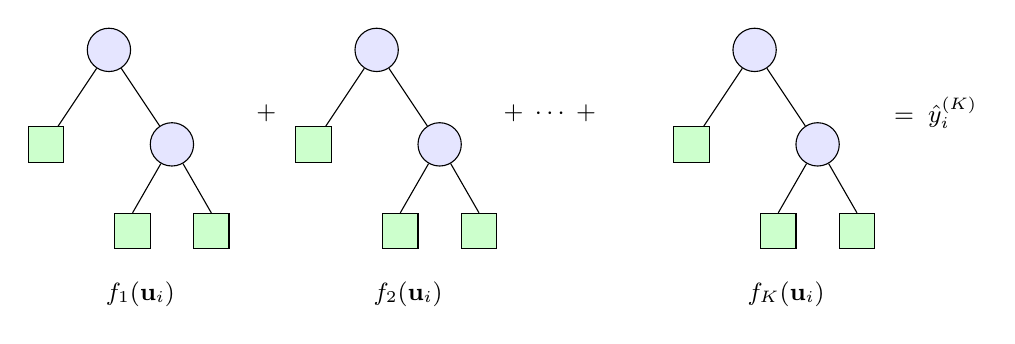
\begin{tikzpicture}[x=1cm,y=1cm,every node/.style={font=\small},
        nd/.style={circle,draw,minimum size=0.55cm,inner sep=0,fill=blue!10},
        lf/.style={rectangle,draw,minimum size=0.45cm,inner sep=0,fill=green!20}]
        \foreach \x/\n in {0/1,3.4/2,8.2/K}{
            \node[nd] (r\n) at (\x,1.2) {};
            \node[lf] (l\n) at (\x-0.8,0) {};
            \node[nd] (m\n) at (\x+0.8,0) {};
            \draw (r\n) -- (l\n);
            \draw (r\n) -- (m\n);
            \node[lf] at (\x+0.3,-1.1) {};
            \node[lf] at (\x+1.3,-1.1) {};
            \draw (m\n) -- (\x+0.3,-0.87);
            \draw (m\n) -- (\x+1.3,-0.87);
            \node at (\x+0.4,-1.9) {\(f_{\n}(\mathbf{u}_i)\)};
        }
        \node at (2.0,0.4) {\(+\)};
        \node at (5.6,0.4) {\(+\;\cdots\;+\)};
        \node at (10.5,0.4) {\(=\;\hat{y}_i^{(K)}\)};
    \end{tikzpicture}
    \caption{Previsão do impulsionamento por gradiente como soma de \(K\) árvores. Cada círculo é uma pergunta sobre um atributo e cada quadrado (folha) guarda um valor. Elaboração própria, com base em \citeonline{chen2016xgboost}.}
    \label{fig:boosting}
\end{figure}

Na Equação~\ref{eq:xgboost_aditivo}, \(f_k\) é a árvore adicionada na etapa \(k\) e \(\mathcal{F}\) é o conjunto de todas as árvores possíveis. O treinamento minimiza o objetivo regularizado da Equação~\ref{eq:xgboost_objetivo}.

\begin{equation}
    \mathcal{L}^{(K)}
    =
    \sum_i \ell(y_i, \hat{y}_i^{(K)})
    +
    \sum_{k=1}^{K}\Omega(f_k),
    \qquad
    \Omega(f_k)=\gamma T_k + \frac{1}{2}\lambda\lVert\mathbf{w}_k\rVert_2^2
    \label{eq:xgboost_objetivo}
\end{equation}

Na Equação~\ref{eq:xgboost_objetivo}, \(\ell\) é a função de perda que compara o valor observado \(y_i\) com a previsão, \(T_k\) é o número de folhas da árvore \(k\), \(\mathbf{w}_k\) é o vetor de valores das folhas, \(\gamma\) penaliza árvores com muitas folhas e \(\lambda\) penaliza valores grandes nas folhas. Esses termos de regularização evitam árvores excessivamente complexas, que ajustariam ruído em vez de padrões.

\section{Treinamento, Perda e Hiperparâmetros}
\label{sec:otimizacao_hpo}

Os \emph{parâmetros} de um modelo, como os pesos de uma rede, são aprendidos no treinamento. Os \emph{hiperparâmetros} são escolhas feitas antes do treinamento, como a taxa de aprendizado, o número de camadas, o tamanho do estado oculto e a profundidade das árvores. O treinamento de uma rede percorre os dados várias vezes; cada passagem completa é uma \emph{época}. O \textit{dropout} desliga aleatoriamente uma fração das unidades da rede a cada passo de treinamento, o que reduz a dependência excessiva de poucas unidades e ajuda a evitar o sobreajuste, isto é, a memorização do treino em vez do aprendizado de padrões gerais \cite{srivastava2014dropout}. O decaimento de pesos (\textit{weight decay}) penaliza pesos grandes com o mesmo objetivo. A parada antecipada interrompe o treinamento quando a medida de erro na validação deixa de melhorar por um número de épocas.

Redes neurais são treinadas com otimizadores baseados em gradiente, como o Adam e o AdamW \cite{kingma2014adam,loshchilov2019decoupled}, que atualizam os parâmetros na direção que reduz a perda. A \emph{taxa de aprendizado} controla o tamanho de cada atualização. Ela pode ser constante ou seguir uma \emph{agenda}, isto é, um plano que a altera ao longo das épocas. Uma agenda comum combina aquecimento linear, em que a taxa cresce no início, e decaimento cosseno, em que ela diminui suavemente depois \cite{goyal2017accurate,loshchilov2017sgdr}. Com \(E_w\) épocas de aquecimento, \(E\) épocas no total, taxa máxima \(\eta_{\max}\) e taxa mínima \(\eta_{\min}\), a taxa na época \(t\) é dada pela Equação~\ref{eq:agenda_taxa_aprendizado}.

\begin{equation}
    \eta_t =
    \begin{cases}
        \eta_{\max}\left(10^{-5} + (1-10^{-5})\frac{t}{E_w}\right), & 0 \leq t \leq E_w,\\
        \eta_{\min} + \frac{1}{2}(\eta_{\max}-\eta_{\min})\left[1+\cos\left(\pi\frac{t-E_w}{E-E_w}\right)\right], & E_w < t \leq E.
    \end{cases}
    \label{eq:agenda_taxa_aprendizado}
\end{equation}

Na Equação~\ref{eq:agenda_taxa_aprendizado}, a primeira linha descreve o aquecimento, em que a taxa cresce de um valor próximo de zero até \(\eta_{\max}\); a segunda descreve o decaimento, em que ela cai suavemente de \(\eta_{\max}\) até \(\eta_{\min}\). A validação não altera os pesos: apenas mede o erro ao fim de cada época.

A escolha da função de perda define o que o modelo procura minimizar. A perda de Huber combina o comportamento quadrático para erros pequenos e linear para erros grandes, o que a torna menos sensível a valores extremos do que a perda quadrática \cite{huber1964robust}. Para o erro \(e=y-\hat{y}\), ela é definida pela Equação~\ref{eq:huber}.

\begin{equation}
    \ell_{\delta}(e)=
    \begin{cases}
        \frac{1}{2}e^2, & \text{se } |e| \leq \delta,\\
        \delta\left(|e|-\frac{1}{2}\delta\right), & \text{caso contrário}.
    \end{cases}
    \label{eq:huber}
\end{equation}

Na Equação~\ref{eq:huber}, \(\delta\) é o limite a partir do qual o erro deixa de ser tratado de forma quadrática. Cada perda tem um valor de previsão que a minimiza: a perda quadrática é minimizada pela média condicional, a perda absoluta pela mediana condicional e a perda de Huber por um valor intermediário \cite{gneiting2011making}. Como a mediana de uma distribuição assimétrica à direita fica abaixo da média, modelos treinados com perda absoluta ou de Huber tendem a subestimar valores altos. A perda também pode ser ponderada, atribuindo peso maior a determinados exemplos, na linha do aprendizado sensível ao custo \cite{elkan2001foundations}.

A busca de hiperparâmetros (\textit{Hyperparameter Optimization}, HPO) automatiza a escolha desses valores. Ajustá-los à mão é trabalhoso, porque muitos interagem entre si e cada teste exige um treinamento completo. Seja \(\kappa \in \mathcal{K}\) uma configuração de hiperparâmetros dentro do espaço de busca \(\mathcal{K}\), e \(A(D_{treino};\kappa)\) o modelo treinado com essa configuração. Em uma validação simples, busca-se a configuração de menor erro de validação, como na Equação~\ref{eq:hpo_objetivo}.

\begin{equation}
    \kappa^{*}
    =
    \arg\min_{\kappa \in \mathcal{K}}
    \mathcal{L}_{val}\left(A(D_{treino};\kappa), D_{val}\right)
    \label{eq:hpo_objetivo}
\end{equation}

Na Equação~\ref{eq:hpo_objetivo}, \(D_{treino}\) e \(D_{val}\) são os dados de treino e de validação, e \(\kappa^{*}\) é a configuração escolhida. Em séries temporais, o erro de validação é substituído pela média entre as partições, \(\mathcal{L}_{CV}\), da Equação~\ref{eq:cv_temporal}. O Optuna é uma ferramenta que realiza essa busca \cite{akiba2019optuna}. Cada \emph{tentativa} (\textit{trial}) testa uma configuração e devolve seu erro; o amostrador \textit{Tree-structured Parzen Estimator} (TPE) usa as tentativas anteriores para propor configurações promissoras \cite{bergstra2011algorithms,optunaDocsTPE2026}. A poda interrompe cedo as tentativas pouco promissoras, poupando tempo: o \textit{Hyperband} distribui o orçamento de treinamento entre muitas configurações e descarta as piores em etapas sucessivas \cite{li2018hyperband}. Uma busca com orçamento limitado não garante encontrar o melhor conjunto possível.

\section{Métricas de Avaliação}
\label{sec:metricas_avaliacao}

Nas equações desta seção, \(N\) é o número de previsões avaliadas, \(y_i\) é o valor observado, \(\hat{y}_i\) é o valor previsto e \(\bar{y}\) é a média dos valores observados. Como a previsão de PM2,5 é uma tarefa de regressão, a qualidade da previsão é medida por meio de erros. O erro médio absoluto (\textit{Mean Absolute Error}, MAE) é a média das diferenças absolutas, como mostra a Equação~\ref{eq:mae}, e tem a mesma unidade da grandeza prevista.

\begin{equation}
    \text{MAE} =
    \frac{1}{N}\sum_{i=1}^{N}|y_i - \hat{y}_i|
    \label{eq:mae}
\end{equation}

A raiz do erro quadrático médio (\textit{Root Mean Squared Error}, RMSE), na Equação~\ref{eq:rmse}, eleva os erros ao quadrado antes da média e, por isso, dá mais peso aos erros grandes.

\begin{equation}
    \text{RMSE} =
    \sqrt{\frac{1}{N}\sum_{i=1}^{N}(y_i - \hat{y}_i)^2}
    \label{eq:rmse}
\end{equation}

O MAE e o RMSE respondem a perguntas diferentes, e reportar os dois evita depender de uma única medida \cite{willmott2005advantages,chai2014rmse}. O erro percentual médio absoluto (\textit{Mean Absolute Percentage Error}, MAPE), na Equação~\ref{eq:mape}, expressa o erro em relação ao valor observado.

\begin{equation}
    \text{MAPE} =
    \frac{100}{N}\sum_{i=1}^{N}\left|\frac{y_i-\hat{y}_i}{y_i}\right|
    \label{eq:mape}
\end{equation}

Como \(y_i\) aparece no denominador, o MAPE cresce muito quando os valores observados são pequenos. Duas medidas percentuais menos sensíveis a isso são o erro percentual absoluto ponderado (\textit{Weighted Absolute Percentage Error}, WAPE) e o MAPE simétrico (sMAPE) \cite{hyndman2006another}, definidos na Equação~\ref{eq:wape_smape}.

\begin{equation}
    \text{WAPE} =
    100\,\frac{\sum_{i=1}^{N}|y_i - \hat{y}_i|}{\sum_{i=1}^{N}|y_i|},
    \qquad
    \text{sMAPE} =
    \frac{100}{N}\sum_{i=1}^{N}\frac{2\,|y_i - \hat{y}_i|}{|y_i| + |\hat{y}_i|}
    \label{eq:wape_smape}
\end{equation}

Na Equação~\ref{eq:wape_smape}, o WAPE é o erro absoluto total dividido pelo total observado, ou seja, o MAE em relação à média das observações; no sMAPE, o termo da soma é considerado zero quando \(y_i=\hat{y}_i=0\). O coeficiente de determinação, \(R^2\), compara o erro do modelo com a variabilidade do próprio alvo, conforme a Equação~\ref{eq:r2}; valores próximos de 1 indicam que o modelo explica boa parte da variação, e valores próximos de 0, que ele não supera a previsão constante igual à média.

\begin{equation}
    R^2 =
    1 - \frac{\sum_{i=1}^{N}(y_i - \hat{y}_i)^2}{\sum_{i=1}^{N}(y_i - \bar{y})^2}
    \label{eq:r2}
\end{equation}

Duas medidas complementares completam o conjunto. O viés médio (\textit{Mean Bias Error}, MBE) é a média de \(\hat{y}_i-y_i\); valores negativos indicam subestimação sistemática. A habilidade (\textit{skill score}) em relação a uma previsão de referência é \(1-\text{MAE}/\text{MAE}_{\text{ref}}\), que é positiva quando o modelo tem erro menor que a referência.

Por fim, o MAE pode ser calculado separadamente para cada horizonte \(h=1,\ldots,H\), como na Equação~\ref{eq:mae_horizonte}.

\begin{equation}
    \text{MAE}_{h} =
    \frac{1}{N_h}\sum_{i=1}^{N_h}|y_{i,h}-\hat{y}_{i,h}|
    \label{eq:mae_horizonte}
\end{equation}

Na Equação~\ref{eq:mae_horizonte}, \(N_h\) é o número de previsões avaliadas para o horizonte \(h\), \(y_{i,h}\) é o valor observado \(h\) instantes após a emissão da previsão \(i\) e \(\hat{y}_{i,h}\) é o valor previsto correspondente. Com isso, é possível ver como o erro cresce à medida que a previsão se afasta do instante de emissão, o que uma média global esconderia.

\section{Comparação Estatística de Previsões}
\label{sec:comparacao_estatistica}

Dois modelos com MAE parecidos podem diferir apenas por acaso da amostra de teste. Para decidir se a diferença é real, é necessário quantificar a incerteza, mas os erros de uma série temporal não são independentes: erros de horas vizinhas tendem a ser parecidos, e as janelas de previsão se sobrepõem. Tratar os erros como independentes subestima a incerteza e produz intervalos estreitos demais.

O \emph{bootstrap em blocos} lida com isso \cite{kunsch1989jackknife,politis1992circular}. Ele repete muitas vezes o seguinte procedimento: sorteia, com reposição, blocos de instantes consecutivos do período de teste (em vez de instantes isolados, o que preserva a dependência dentro de cada bloco) e recalcula a diferença de erro entre os dois modelos, usando os mesmos blocos para ambos. As diferenças obtidas formam uma distribuição, e os percentis 2,5\% e 97,5\% dessa distribuição delimitam um intervalo de confiança de 95\% para a diferença. Se o intervalo contém o zero, não há evidência estatística de que um modelo seja melhor que o outro.

O teste de Diebold-Mariano \cite{diebold1995comparing} é uma alternativa que compara diretamente as perdas. Sendo \(d_o\) a diferença entre a perda do modelo A e a do modelo B na previsão \(o\), a estatística do teste é a média das diferenças dividida pelo seu erro-padrão, como na Equação~\ref{eq:dm}.

\begin{equation}
    DM=\frac{\bar{d}}{\sqrt{\widehat{V}(\bar{d})}}
    \label{eq:dm}
\end{equation}

Na Equação~\ref{eq:dm}, \(\bar{d}\) é a média das diferenças de perda, e \(\widehat{V}(\bar{d})\) é uma estimativa da variância dessa média que leva em conta a autocorrelação das diferenças, como a de \citeonline{newey1987simple}. A correção de \citeonline{harvey1997testing} ajusta o teste para amostras finitas. Valores de DM distantes de zero (valor-\(p\) pequeno) indicam que as previsões têm qualidade diferente. O bootstrap fornece o intervalo na unidade da métrica, e o teste fornece um valor-\(p\) sob suposições assintóticas; por isso, os dois se complementam.
